\chapter{Theoretical background}
%Here you identify and give the theoretical background needed in this report, with proper references to each literature reference used. The selection of what to include should be discussed and agreed with the supervisors. Theory may involve concepts, definitions, methods, regulations/key standards, theory to explain specific system behavior, and so on.
In this chapter we are going to investigate some of the key concepts related to pattern recognition and shape detection in imagery. 

\section{Shape detection}
Identifying geometric shapes in computer vision has been a classical problem for decades. There are many theories related to what is the best way of detecting a particular shape in an image, with shapes defines as two dimensional features of an object that are invariant to scene factors, or whose variation can be modeled easily \citep{Moon2002}.

\subsection{The standard approach}
Most images are based on a raster format, meaning that pixels in the image are structured as an array or grid, where each pixel is associated with a position (row and column), and a numeric value. Raster images can represent a range of different shapes, where a point can be represented by a single pixel and a circle by a contiguous collection of pixels \citep{Worboys2003}. Even though rasters are easy to work with in most computer systems, since they are represented the way that they are, they do not contain any information about the topology of the objects in the image. For example, there is no way of knowing if a pixel is contained within a certain object or not. In order to identify objects, one approach is therefore to detect edge pixels.

There are many well-known methods that are used in order to find an objects external contour, such as the generalized Hough transform (GHT) \citep{Ballard1981}, fitting of polynomial curves and applying band matching after edge detection.

In recent years shape detection algorithms have come to increasingly rely on superpixel algorithms, which groups pixels into perceptually meaningful atomic regions \citep{Achanta2012}. Such regions replace the regular, rigid structure of the raster grid, as shown in \autoref{fig:superpixels}.

\begin{figure}[!h]
	\centering
	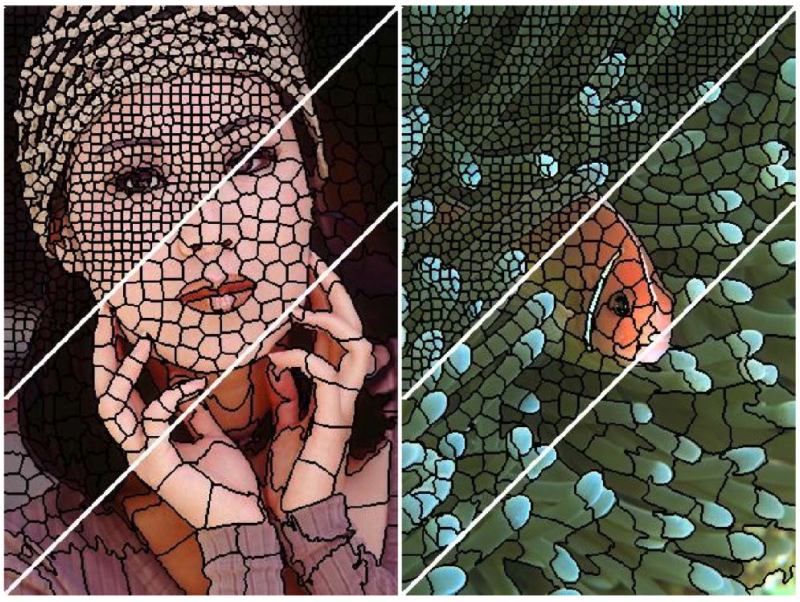
\includegraphics[scale=0.3]{fig/superpixels}
	\caption{Visualization of image segmentation using SLIC \citep{Achanta2012}}
	\label{fig:superpixels}
\end{figure}

When constructing superpixels, there are some properties of the algorithm that are desirable, regardless of the problem that are being solved. These are, according to \citep{Achanta2012}, the following three points:

\begin{itemize}
	\item Superpixels should adhere well to image boundaries
	\item When used to reduce computional complexity as a preprocessing step, superpixels should be fast to compute, memory efficient, and simple to use.
	\item When used for segmentation purposes, superpixels should both increase the speed and improve the quality of the results.
\end{itemize}

\cite{Achanta2012} proposes a superpixel-segmentation algorithm (SLIC), which in their opinion is best suited to meet these demands. They compare their algorithm to a variety of state-of-the-art superpixel methods, and conclude that none of the existing methods are satisfactory in regards to the points.

\subsubsection*{Simple Linear Iterative Clustering (SLIC)}
The SLIC algorithm is fairly simple to understand. One of its key principles is that, by limiting the search space for each cluster center (points in the regular raster grid), it reduces the search speed significantly. This is achievable due to the fact that one of the primary goals of algorithm is to create a set of approximately equal sized superpixels. Thus, instead of searching the whole raster grid for each cluster center, the algorithm only has to search for edge pixels at a distance equal to D, as shown in \autoref{eq:distanceSuperpixel}.

\begin{equation}
	D'=\sqrt{\left(\frac{d_{c}}{m}\right)^{2} + \left(\frac{d_{s}}{S}\right)^{2}}
	\label{eq:distanceSuperpixel}
\end{equation}

In \autoref{eq:distanceSuperpixel} $d_{c}$ is the euclidean distance between two pixels in terms of color and $d_{s}$ is the pixels euclidean, spatial distance. Furthermore, $S$ is the sampling interval of the cluster centers ($S = \sqrt{N/k}$, where N is the number of pixels in the grid and k is the desired number of superpixels) and $m$ is a fixed constant based on the color diversity in the image.

Since the algorithm generates superpixels by clustering pixels based on their color and spatial proximity, creating a 5 dimensional, \textit{labxy} space, one would think that the distance could be found by simply taking the 5D euclidean distance. However, it turns out that for large superpixels, spatial distance outweigh the color proximity. Which is why the two distances $d_{c}$ and $d_{s}$ are weighted.

\subsection{The cognitive approach}
In recent years, the development of machine learning, a branch of artificial intelligent systems, has become increasingly important in terms of pattern and object recognition in remote sensing and image analysis in general.

\cite{Lary2016} propose nine different branches of machine learning that are commonly used for data mining in remote sensing. These algorithms are artificial neural networks (ANN), support vector machines (SVM), self-organizing map (SOM), decision trees (DT), ensemble methods such as random forests, case-based reasoning, neuro-fuzzy (NF), generic algorithm (GA) and multivariate adaptive regression splines (MARS). In particular, three of these algorithms are of interest.

\subsubsection*{Artificial Neural Networks}
The basic principle behind artificial neural networks (ANNs) is that it is built up by a network of many simple units that are working in parallel with no centralized control unit. The networks primary means of storage are the weights between the individual units, and the network learns by updating these weights in relation to being provided with a training example.

In order to understand the behavior of ANNs it is important to understand their structure. An ANN is build up by a given number of connected layers. A layer is a collection of simple units, called artificial neurons. All ANNs must consist of an input and output layer, but can also contain an optional number of hidden layers. A network which only consists of an input and output layer is called a perceptron.

\subsubsection*{Support vector machines}
In machine learning, support vector machines (SVM) are supervised learning models used for classification and regression analysis.

In a SVM model training examples are represented as points in a n-dimensional space, mapped so that the examples belonging to separate categories are clustered together. One or more hyperplanes are then fitted in order to separate the different classes from each other. New data is then mapped into that same space and classified based on which side of the hyperplane they are mapped. SVMs are often called large margin classifiers because their goal is to separate the classes by fitting the hyperplanes between them in a way so that the planes has the highest possible margin between the classes as shown in \autoref{fig:optimalmargin}.

\begin{figure}[!h]
	\centering
	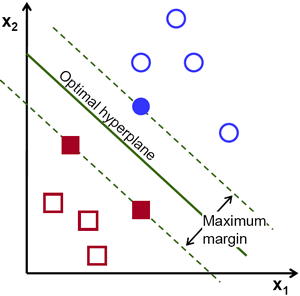
\includegraphics[scale=2.5]{fig/optimal-hyperplane.png}
	\caption{Example of optimal hyperplane for classification from \cite{Opencv2017}}
	\label{fig:optimalmargin}
\end{figure}

In order for support vector machines to work, the data points has to be separable by a plane. This is however not always possible in the dimension that the data is represented. In order to solve this issue SVM apply kernel functions.

Kernel functions enable SVM to operate in a high-dimensional, implicit feature space without ever computing the coordinates of the data in that dimension space. It simply computes the inner products between the images of all pairs of data in the feature space. This operation is often computationally cheaper than the explicit computation of the coordinates.

\begin{figure}[!h]
	\centering
	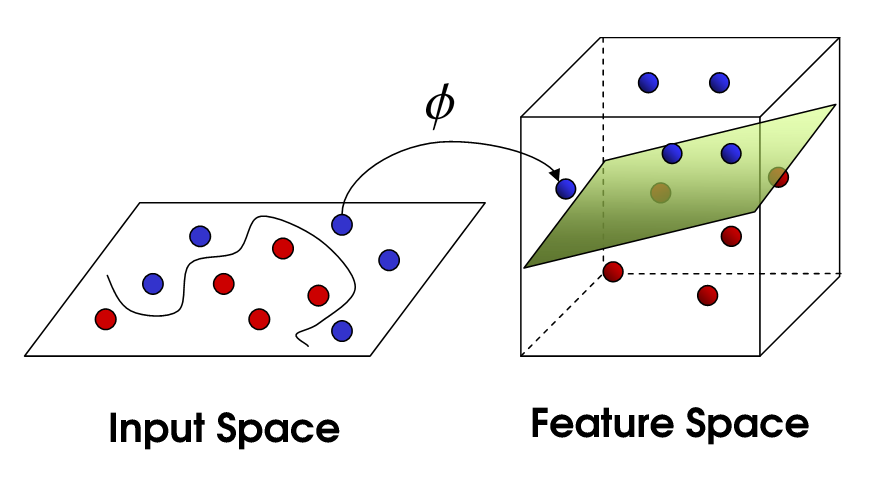
\includegraphics[scale=0.3]{fig/kernel_function.png}
	\caption{Classification using SVM with kernel function \cite{Opencv2017}}
	\label{fig:kernerlfunction}
\end{figure}

\subsubsection*{Decision Trees}
Decision tree learning is one of the simplest and yet most successful forms of machine learning. They are learned top-down, and they use a recursive learning technique.

A decision tree represents a function that takes as input a vector of attribute values and returns a “decision” - a single output value. Furthermore, it is worth mentioning that decision trees are only good for some kind of functions.

Links:

https://www.pyimagesearch.com/2014/10/20/finding-shapes-images-using-python-opencv/\\
https://www.pyimagesearch.com/2016/02/08/opencv-shape-detection/
\\
http://melvincabatuan.github.io/SLIC-Superpixels/
\\
